% generated by scripts/pkl_to_latex.py
% source PKL : uscan_v1_L6_Ne6_t0p1_mode-uniform_nmin2_solver-gcg_full_restarts2_iter200_kmax4_tol1em09_U1to20_N20-d03a74da789e.pkl
% scan type  : uscan
% state      : gs
% requires   : \usepackage{pgfplots} \pgfplotsset{compat=1.18}
% colours match the matplotlib PDF (tab10 cycle)
\definecolor{gmeC0}{HTML}{1F77B4}
\definecolor{gmeC1}{HTML}{FF7F0E}
\definecolor{gmeC2}{HTML}{2CA02C}
\definecolor{gmeC3}{HTML}{D62728}
\definecolor{gmeC4}{HTML}{9467BD}
\definecolor{gmeC5}{HTML}{8C564B}
\definecolor{gmeC6}{HTML}{E377C2}
\definecolor{gmeC7}{HTML}{17BECF}

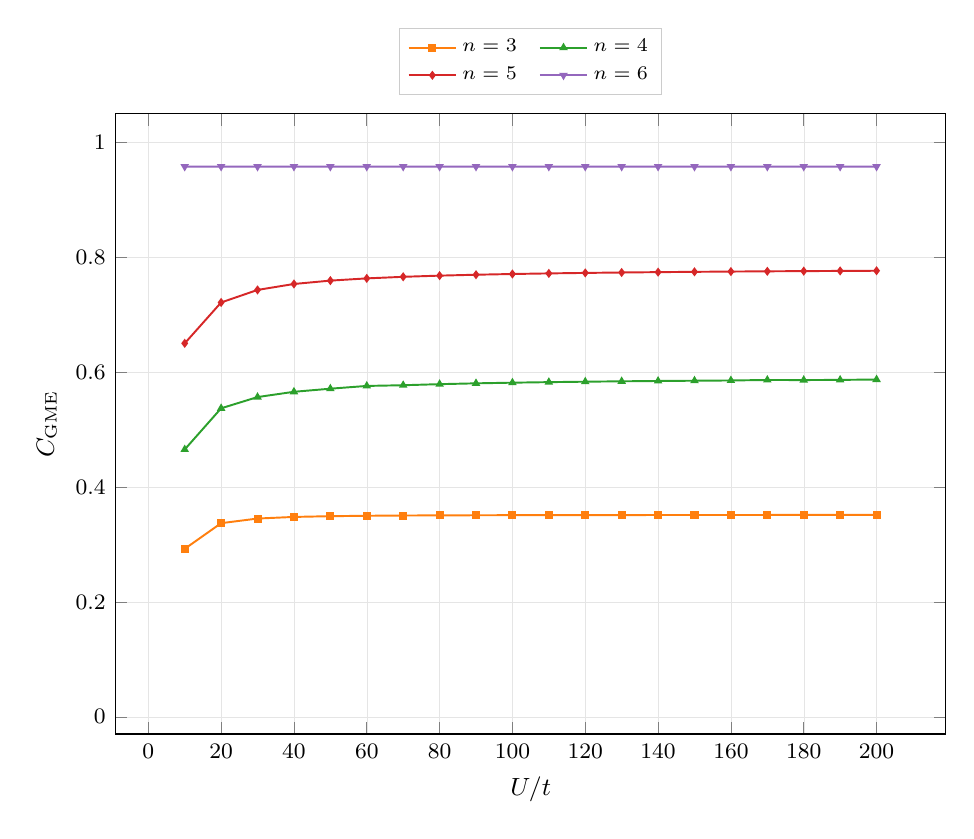
\begin{tikzpicture}
  \begin{axis}[
    width=\columnwidth,
    height=0.78\columnwidth,
    xlabel={$U/t$},
    ylabel={$C_{\mathrm{GME}}$},
    grid=both,
    grid style={line width=.1pt, draw=gray!20},
    tick label style={font=\footnotesize\rmfamily, /pgf/number format/fixed},
    label style={font=\small\rmfamily},
    scaled ticks=false,
    legend style={font=\scriptsize\rmfamily, draw=gray!40, at={(0.5,1.03)}, anchor=south, /tikz/every even column/.append style={column sep=6pt}},
    legend cell align={left},
    legend columns=2,
    ymin=-0.03,
    ymax=1.05,
  ]
    \addplot[color=gmeC1, mark=square*, mark size=1.1pt, line width=0.7pt] coordinates {
        (10,0.292503) (20,0.337214) (30,0.345268) (40,0.348079)
        (50,0.349379) (60,0.350086) (70,0.350511) (80,0.350788)
        (90,0.350977) (100,0.351113) (110,0.351213) (120,0.351289)
        (130,0.351349) (140,0.351396) (150,0.351434) (160,0.351465)
        (170,0.351491) (180,0.351512) (190,0.351531) (200,0.351546)
    };
    \addlegendentry{$n=3$}
    \addplot[color=gmeC2, mark=triangle*, mark size=1.1pt, line width=0.7pt] coordinates {
        (10,0.465524) (20,0.537235) (30,0.556812) (40,0.566001)
        (50,0.571386) (60,0.576213) (70,0.577415) (80,0.579277)
        (90,0.580719) (100,0.581864) (110,0.582801) (120,0.58358)
        (130,0.584239) (140,0.584817) (150,0.585286) (160,0.585711)
        (170,0.58655) (180,0.586418) (190,0.586716) (200,0.587379)
    };
    \addlegendentry{$n=4$}
    \addplot[color=gmeC3, mark=diamond*, mark size=1.1pt, line width=0.7pt] coordinates {
        (10,0.650353) (20,0.721531) (30,0.743387) (40,0.753744)
        (50,0.759606) (60,0.763475) (70,0.766221) (80,0.768269)
        (90,0.769856) (100,0.771122) (110,0.772154) (120,0.773013)
        (130,0.773739) (140,0.77436) (150,0.774897) (160,0.775367)
        (170,0.775781) (180,0.776148) (190,0.776477) (200,0.776773)
    };
    \addlegendentry{$n=5$}
    \addplot[color=gmeC4, mark=triangle*, mark size=1.1pt, mark options={rotate=180}, line width=0.7pt] coordinates {
        (10,0.958182) (20,0.958179) (30,0.958179) (40,0.958179)
        (50,0.958179) (60,0.958179) (70,0.958179) (80,0.958179)
        (90,0.958179) (100,0.958179) (110,0.958179) (120,0.958179)
        (130,0.958179) (140,0.958179) (150,0.958179) (160,0.958179)
        (170,0.958179) (180,0.958179) (190,0.958179) (200,0.958179)
    };
    \addlegendentry{$n=6$}
  \end{axis}
\end{tikzpicture}
